\documentclass[12pt]{article}
\usepackage[utf8]{inputenc}
\usepackage{graphicx} 
\usepackage{wrapfig}
\usepackage[dvipsnames]{xcolor}
\usepackage{moreverb}
\usepackage{ragged2e}
\renewcommand\refname{Referencias}
\title{Elementos de la programación Python 1.}
\author{\textcolor{JungleGreen}{Olga María Fimbres Morales}}
\date{17 de Enero 2016}
\begin{document}
\begin{titlepage}

\begin{center}
\begin{large}
Universidad del Estado de Sonora\\
\end{large}
\vspace*{0.15in}
División de Ciencias Exactas y Naturales.\\
\vspace*{0.15in}
Licenciatura en Física. \\
\vspace*{0.6in}
\begin{large}
Física Computacional 1\\
\end{large}
\vspace*{0.2in}
\begin{Large}
\textbf{{\textcolor{Red}{Animaciones con Matplotlib.}}} \\
\end{Large}

%\begin{Large}
%\textbf{{\textcolor{Red}{Péndulo.}}} \\
%end{Large}
%\vspace*{-1in}

\rule{80mm}{0.1mm}\\
\vspace*{0.1in}
\begin{large}
{\textcolor{JungleGreen}{Olga María Fimbres Morales}}\\
29 de Abril de 2016\\
\end{large}
\end{center}
\end{titlepage}

\pagebreak
\section*{Introducción.}
 Retomando nuestro estudio sobre el modelo f\'isico del p\'endulo simple completamos nuestro análisis del mismo desarrollando ahora una animación del modelo; así como una animación simultanea de cada escenario en el espacio fase, para mostrar de esta forma como es que se relacionan su posición y velocidad angular.\\

Esto se desarrollo con ayuda de la herramienta Matplotlib que nos permite generar animaciones de diferentes escenarios por medio de las expresiones matemáticas adecuadas; dándonos además una gran libertad en el trato de la estética de las mismas, lo que permite al usuario construir una presentación adecuada para diferentes fines.\\

Una vez comprendida la forma en que se utilizan las ecuaciones ya conocidas sobre el movimiento del péndulo simple desarrollaremos de una forma sencilla la manera adecuada para crear archivos mp4 desde Python y de esta forma ser capaces de crear y guardas nuestras propias animaciones. 
 
\section*{\textcolor{Red}{Matplotlib.}}
Matplotlib es una biblioteca de Python de gráficas en 2D que nos proporciona diferentes ejemplos interactivos utilizando diversas herramientas de graficación.\\

Permite al una gran libertad de control sobre el aspecto que tendrá la animación desde el tamaño de los ejes, el estilo de línea, colores, etc. Dejando así todo a la imaginación del usuario para cubrir sus necesidades en cuanto a la estética que desea en su modelo, por ejemplo el poner mas de una animación a la vez para lograr mejor su objetivo de transmitir su idea.\\

Las diferentes herramientas que utiliza son variados, pero resaltan dos para proyección y mapeo, que sonbasemap y cartopy, los cuales puedes instalas fácilmente. Estos son paqueterías diseñadas para realizar dibujos de mapas por medio de análisis de datos, permitiéndonos de este modo visualizar características de una forma mucho más sencilla.\\

Siendo de esta forma un importante recurso ya que estimula la comprensión del fenómeno que estamos desarrollando de una forma más interactiva. Por lo que resulta importante conocer la manera en que podemos trabajar con animaciones, así como los alcances que tenemos con estas, ya que es posible incluso generar alguna de un fenómeno diferente a los acostumbrados, como lo son los aleatorios.

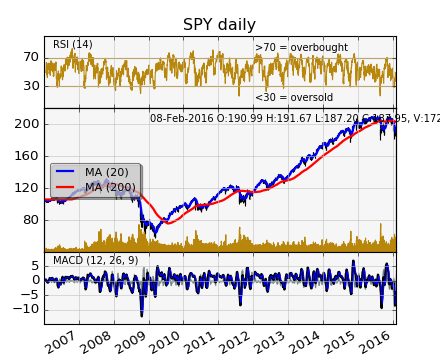
\includegraphics[scale=0.8]{Act10.png}

\pagebreak
\section*{\textcolor{LimeGreen}{Problema.}}

Para el desarrollo de esta actividad se nos proporcionó inicialmente un programa que desarrolla las soluciones a las ecuaciones del péndulo doble y que además realiza una animación del mismo fenómeno, mismo que se agrega en la sección de anexos. Este programa ya se encuentra desarrollado en su totalidad por lo que solo procedió a adaptarse al escenario que nos interesaba para esta actividad.\\

Para ello era necesario eliminar el segundo brazo del péndulo para tener de vuelta el modelo del péndulo simple, por lo que en lugar de eliminar del código original todo aquello correspondiente a este segundo péndulo. Buscando la menor alteración posible y con ello el menor porcentaje de fallo, simplemente se optó por cambiar la longitud del segundo brazo a $0 m$ y de esta forma ser posible ignorar todo lo concerniente a este mismo.\\

En seguida se decidió suprimir todo aquello que tuviera que ver con la energía del péndulo, ya que el código original permitía este calculando mostrándolo además en la animación.\\

Una vez realizados todos estos cambios se tiene un código un poco más sencillo, añadido también en la sección de anexos. Sin embargo, una vez analizado el código se nota que no se realiza un guardado de datos como normalmente estuvimos trabajando con anterioridad, por lo que para cumplir con el segundo objetivo de la práctica, el cual es realizar una animación de diferentes escenarios del péndulo simple dentro del espacio fase, no resulta útil este código.\\

Es por esto, que se recurrió a actividades anteriores donde se desarrollara un programa que realizara los cálculos de velocidades y posiciones angulares para distintos escenarios que pudieran ser guardados y reutilizados dentro de otro programa. En una primera prueba se recurrió al código de la Actividad 7, la cual consistió en el desarrollo del espacio fase del péndulo, sin embargo se tuvieron algunos problemas una vez se llegaba a una cierta condición en especial y la simulación resultaba incorrecta con el modelo físico.\\

La segunda opción fue la Actividad 5, en la cual calculamos íntegramente posición y velocidad angular con el fin de desarrollar una gráfica que tuviera ambas descripciones del péndulo.\\

\begin{boxedverbatim}
#theta'(t) = omega(t)
#omega'(t) = -b*omega(t) - c*sin(theta(t))

def pend(y, t, b, c):
     theta, omega = y
     dydt = [omega, -b*omega - c*np.sin(theta)]
     return dydt

b = 0.4 #fricción
g = 9.8 #gravedad
l = 4.5 #longitud de la cuerda
c = g/l

y0 = [np.pi/3, 0.9] #ángulo inical, velocidad angular

t = np.linspace(0, 20, 500) #rango de tiempo

from scipy.integrate import odeint
sol = odeint(pend, y0, t, args=(b, c))

import matplotlib.pyplot as plt
plt.plot(t, sol[:, 0], 'b', label='posicion(t)') 
#theta = posición
plt.plot(t, sol[:, 1], 'g', label='velocidad(t)')
#omega = velocidad angular
plt.legend(loc='best')
plt.xlabel('Tiempo')
plt.grid()
plt.show()
\end{boxedverbatim}


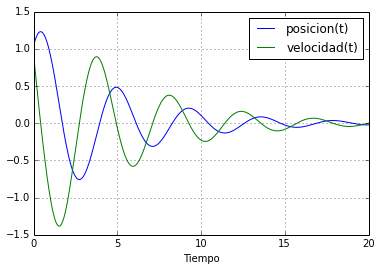
\includegraphics{Act102.png}

Una vez contando con los datos se procedió a realizar cada uno de los escenarios deseados mientras los datos arrojados por el código anterior eran guardados en diferentes archivos creados dentro del código que mas tarde se utilizarían dentro del código correspondiente al espacio fase animado.\\

\begin{boxedverbatim}
file = open("act10150V.txt","w")
file.close()
file = open('act10150V.txt','r')

#Crear archivo a partir de los datos obtenidos
savetxt("act10150V.txt", sol)
\end{boxedverbatim}
\\

Podemos ver como el nombre puede ser modificado conforme se necesite y de esta forma tener guardados diferentes escenarios dentro del mismo programa sin necesidad de realizar documentos dentro de nuestra computadora que mas tarde se abrirán dentro del programa.\\

Después de esto vuelve a abrirse el archivo para especificar una variable a cada columna contenida, además como medio preventivo y para reducir las probabilidades de fallo se guardan nuevamente especificando que se trata de datos numéricos.\\

\begin{center}
\begin{boxedverbatim}
import matplotlib.pyplot as plt 
import numpy as np

data = np.loadtxt('act10170.txt')

x1=data[:,0] #velocidad angular
y1=data[:,1] #posición angular


#convertir es archivo a datos
x11 = x1.astype(np.float) #velocidad
y11 = y1.astype(np.float) #posición
\end{boxedverbatim}
\end{center}

Finalmente, estas últimas variables se utilizan para formar la animación del espacio fase, recordando de cambiar el archivo cada vez que se desee correr un nuevo espacio fase. Programa que se obtuvo a partir de un ejemplo tomado de la biblioteca de animaciones de Matplotlib, mismo que se adjunta en los anexos, y el cual realizada la animación de los tres diferentes planos $xy, xz$ y $yz$ para la función especificada en cada uno de sus ejes.\\

De esta forma se ignoró todo lo que tuviera que ver con dos de los tres planos, conservando únicamente la animación del plano $xy$; así, las últimas variables definidas a partir de los archivos que contiene los datos, es decir $x11$ y $y11$, se utilizan ahora para definir las funciones de los ejes $x$ y $y$, respectivamente. Además de esto se decidió a realizar una reorganización de la animación, así como los colores utilizados y el tamaño de los ejes. Obteniendo de esta forma el espacio fase animado para cada uno de los escenarios deseados.\\

Finalmente, se realizó una integración con ambas animaciones al mismo tiempo para generar la imagen GIF del péndulo con cada una de las condiciones generadas, mismas que se agregan al repositorio Github.






  







\pagebreak

\section*{\textcolor{RoyalBlue}{Resultados}}
Una vez que conseguimos que los programas funcionen de manera adecuada, lo único que resta por hacer es dar las condiciones iniciales que deseamos y generar nuestras animaciones. Se desarrollados 9 diferentes escenarios, los cuales se muestras a continuación.\\
\begin{center}
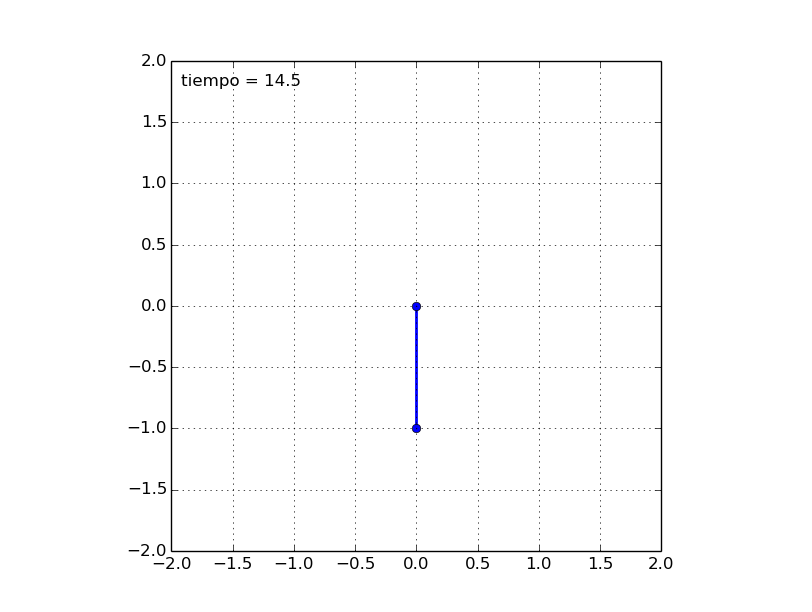
\includegraphics[scale=0.5]{0.png}\\
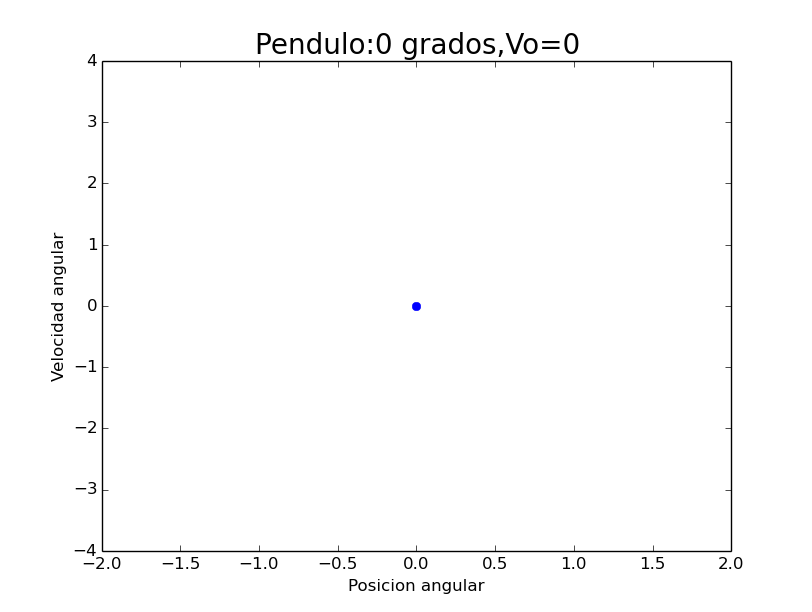
\includegraphics[scale=0.5]{figure_2.png}
\end{center}

\begin{center}
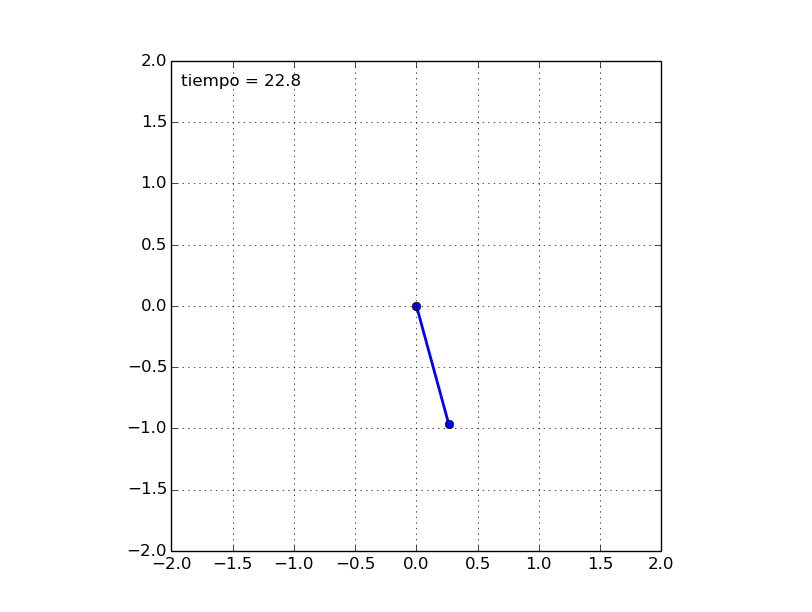
\includegraphics[scale=0.5]{30.png}\\
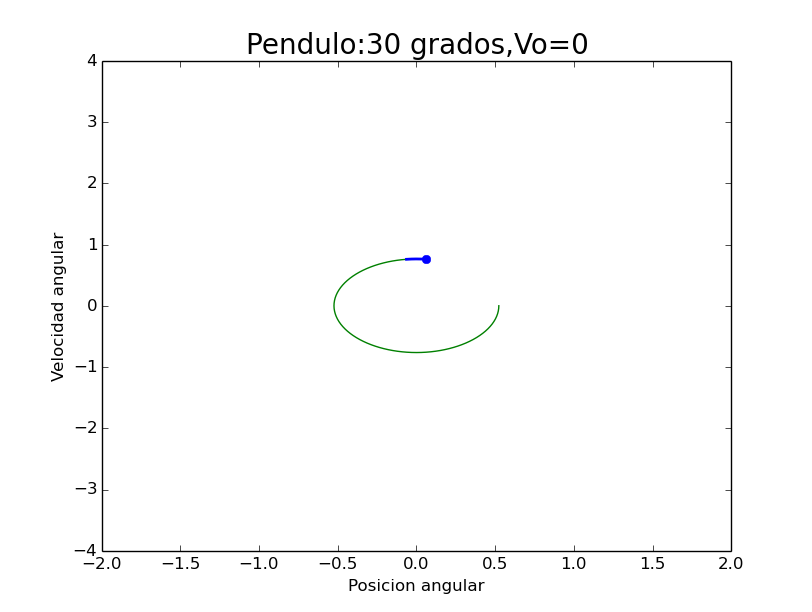
\includegraphics[scale=0.5]{figure_30.png}
\end{center}

\begin{center}
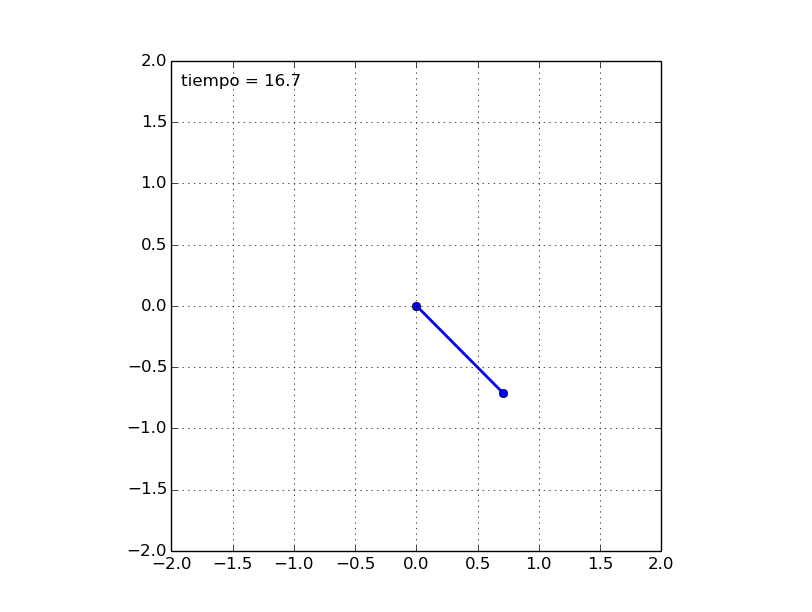
\includegraphics[scale=0.5]{45.png}\\
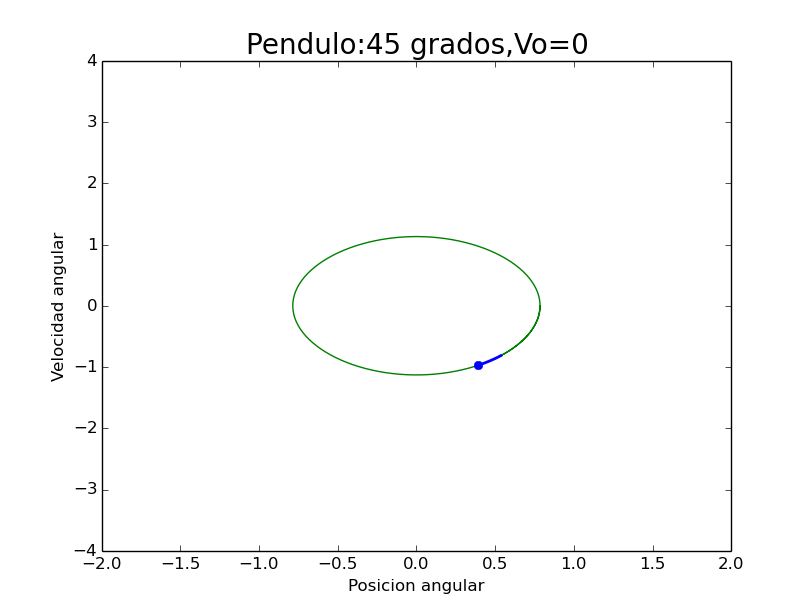
\includegraphics[scale=0.5]{45fase.png}
\end{center}

\begin{center}
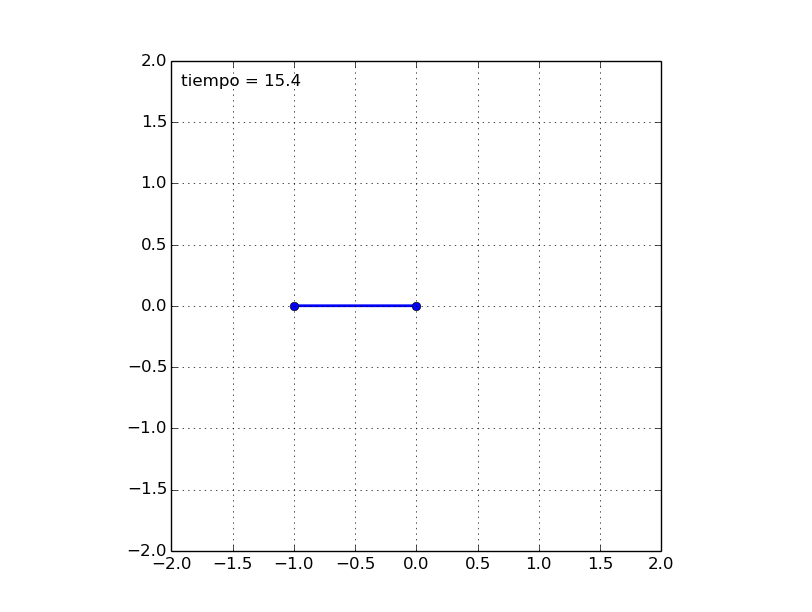
\includegraphics[scale=0.5]{90.png}\\
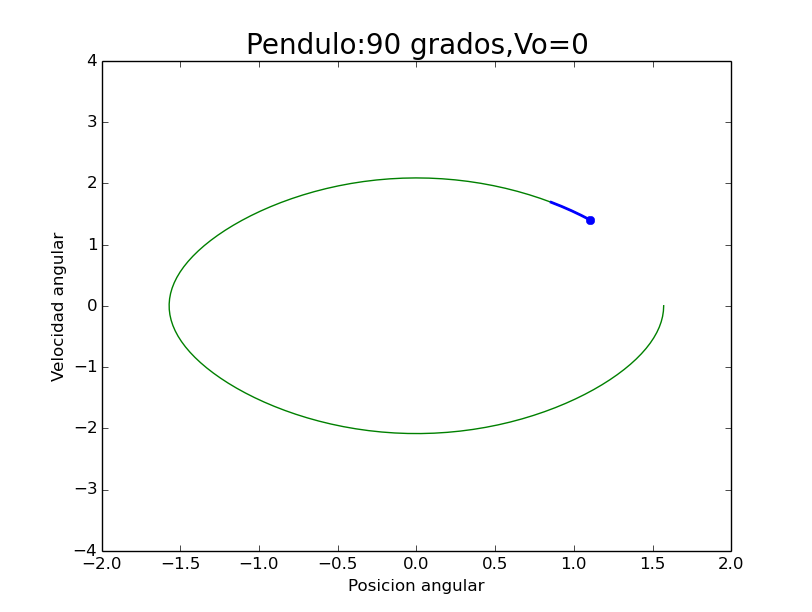
\includegraphics[scale=0.5]{figure_90.png}
\end{center}

\begin{center}
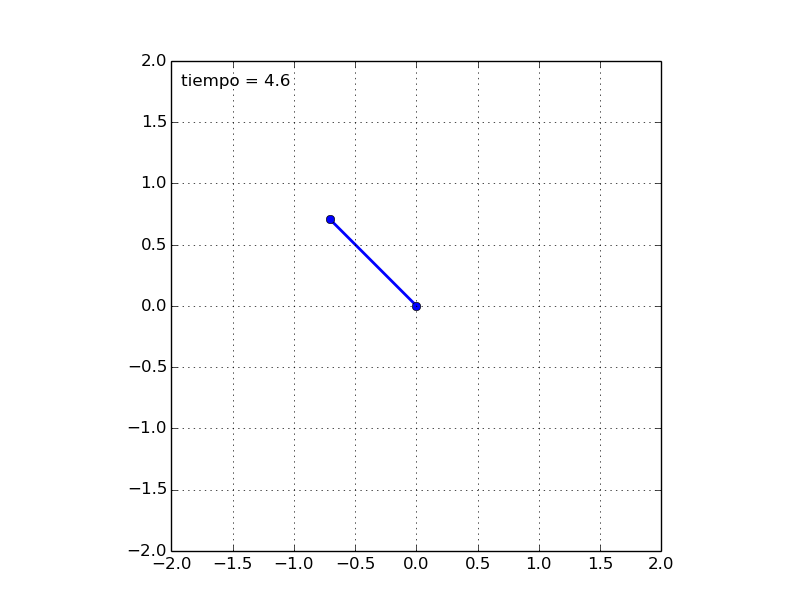
\includegraphics[scale=0.5]{135.png}\\
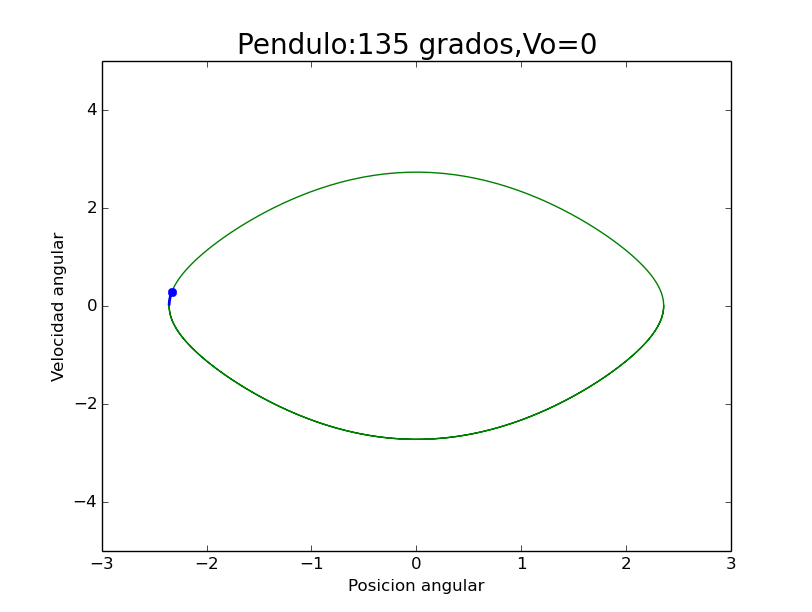
\includegraphics[scale=0.5]{figure_135.png}
\end{center}

\begin{center}
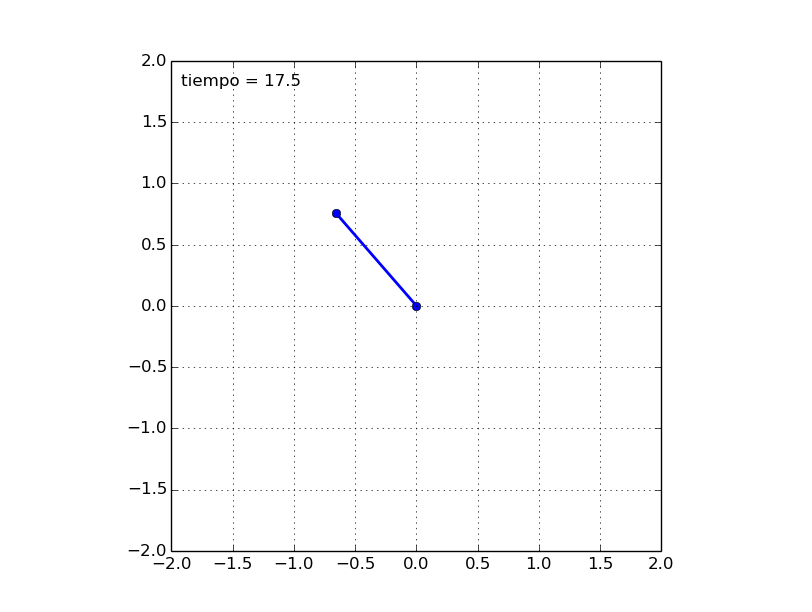
\includegraphics[scale=0.5]{150v.png}\\
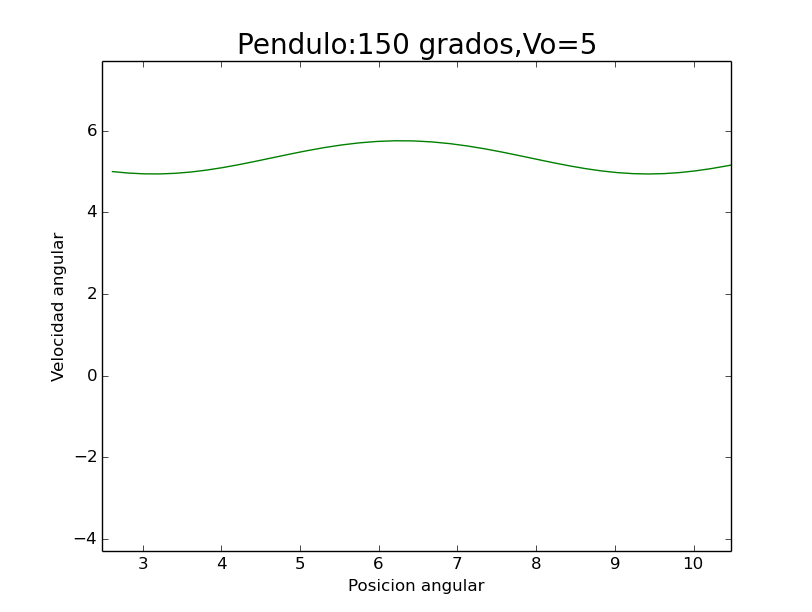
\includegraphics[scale=0.5]{figure_150v.png}
\end{center}

\begin{center}
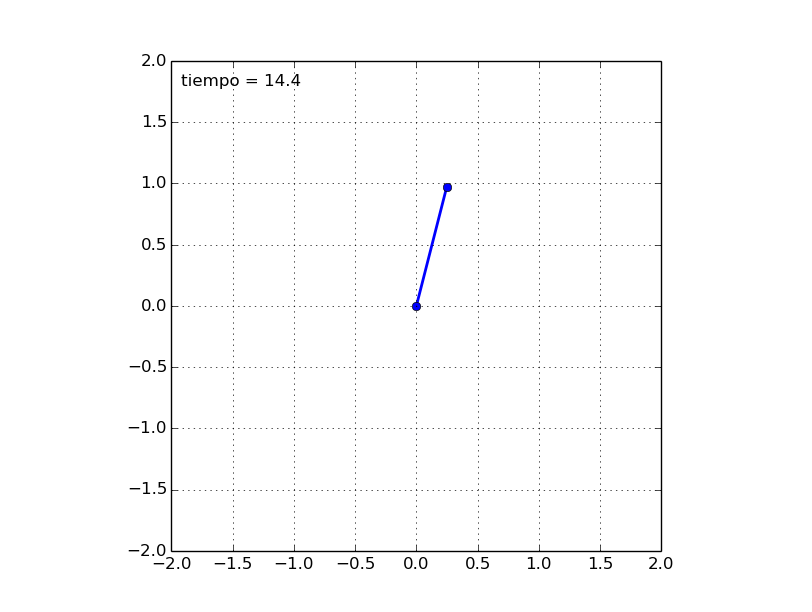
\includegraphics[scale=0.5]{170.png}\\
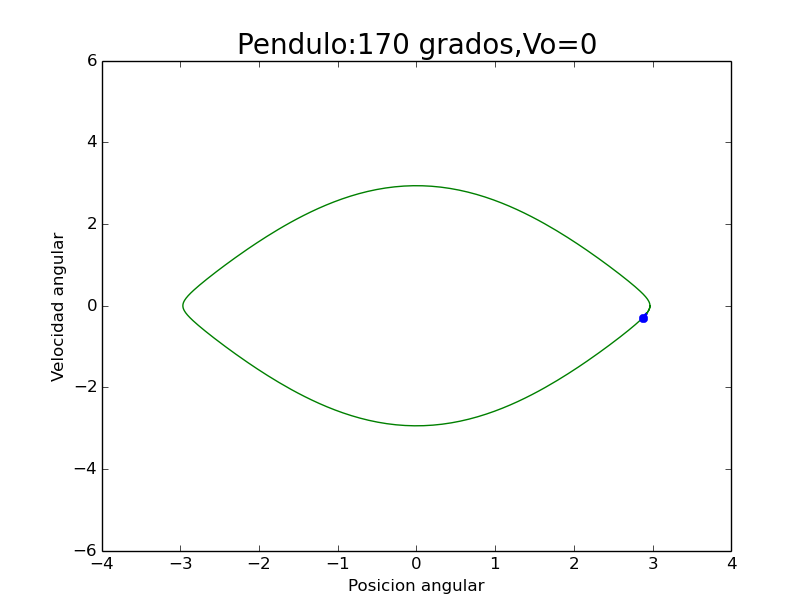
\includegraphics[scale=0.5]{figure_170.png}
\end{center}

\begin{center}
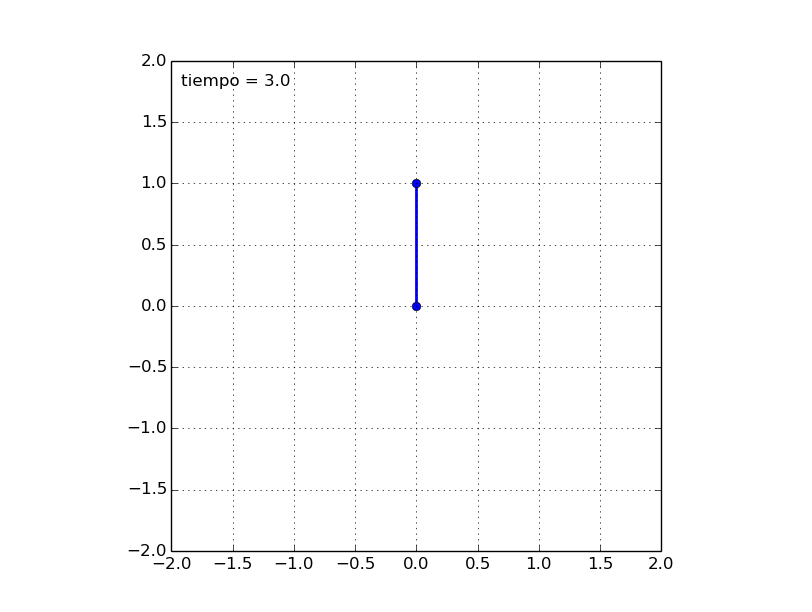
\includegraphics[scale=0.5]{180.png}
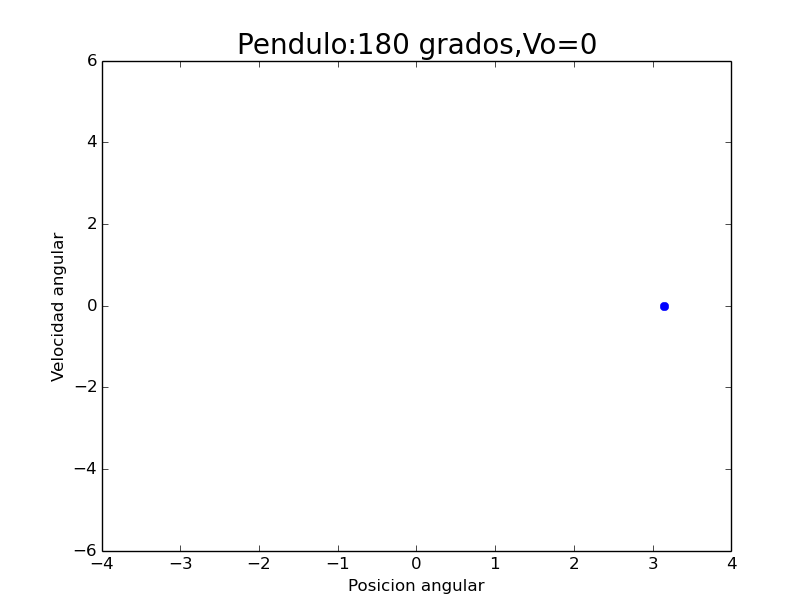
\includegraphics[scale=0.5]{figure_180.png}
\end{center}
Podemos ver que de esta forma resulta sencillo relacionar una imagen de espacio fase con el movimiento que el péndulo realiza; permitiéndonos de este modo tener una visión mucho más amplia y enriquecida del modelo del péndulo simple.

\pagebreak
\section*{\textcolor{Purple}{Anexos}}
\subsection*{\textcolor{RubineRed}{Código Péndulo Doble.}}
\begin{center}
\begin{boxedverbatim}
from numpy import sin, cos
import numpy as np
import matplotlib.pyplot as plt
import scipy.integrate as integrate
import matplotlib.animation as animation

class DoublePendulum:
    """Double Pendulum Class

    init_state is [theta1, omega1, theta2, omega2] in degrees,
    where theta1, omega1 is the angular position and velocity of the first
    pendulum arm, and theta2, omega2 is that of the second pendulum arm
    """
    def __init__(self,
                 init_state = [120, 0, -20, 0],
                 L1=1.0,  # length of pendulum 1 in m
                 L2=1.0,  # length of pendulum 2 in m
                 M1=1.0,  # mass of pendulum 1 in kg
                 M2=1.0,  # mass of pendulum 2 in kg
                 G=9.8,  # acceleration due to gravity, in m/s^2
                 origin=(0, 0)): 
        self.init_state = np.asarray(init_state, dtype='float')
        self.params = (L1, L2, M1, M2, G)
        self.origin = origin
        self.time_elapsed = 0

        self.state = self.init_state * np.pi / 180.
    
    def position(self):
        """compute the current x,y positions of the pendulum arms"""
        (L1, L2, M1, M2, G) = self.params

        x = np.cumsum([self.origin[0],
              L1 * sin(self.state[0]),
              L2 * sin(self.state[2])])
        y = np.cumsum([self.origin[1],
              -L1 * cos(self.state[0]),
              -L2 * cos(self.state[2])])
         return (x, y)
\end{boxedverbatim}
\end{center}

\pagebreak
\begin{boxedverbatim}                       
def energy(self):
        """compute the energy of the current state"""
        (L1, L2, M1, M2, G) = self.params

        x = np.cumsum([L1 * sin(self.state[0]),
                       L2 * sin(self.state[2])])
        y = np.cumsum([-L1 * cos(self.state[0]),
                       -L2 * cos(self.state[2])])
        vx = np.cumsum([L1 * self.state[1] * cos(self.state[0]),
                        L2 * self.state[3] * cos(self.state[2])])
        vy = np.cumsum([L1 * self.state[1] * sin(self.state[0]),
                        L2 * self.state[3] * sin(self.state[2])])

        U = G * (M1 * y[0] + M2 * y[1])
        K = 0.5 * (M1 * np.dot(vx, vx) + M2 * np.dot(vy, vy))

        return U + K
 def dstate_dt(self, state, t):
         """compute the derivative of the given state"""
         (M1, M2, L1, L2, G) = self.params
 
         dydx = np.zeros_like(state)
         dydx[0] = state[1]
         dydx[2] = state[3]
 
         cos_delta = cos(state[2] - state[0])
         sin_delta = sin(state[2] - state[0])
 
         den1 = (M1 + M2) * L1 - M2 * L1 * cos_delta * cos_delta
         dydx[1] = (M2 * L1 * state[1] * state[1] * sin_delta * cos_delta
                    + M2 * G * sin(state[2]) * cos_delta
                    + M2 * L2 * state[3] * state[3] * sin_delta
                    - (M1 + M2) * G * sin(state[0])) / den1
 
         den2 = (L2 / L1) * den1
         dydx[3] = (-M2 * L2 * state[3] * state[3] * sin_delta * cos_delta
                    + (M1 + M2) * G * sin(state[0]) * cos_delta
                    - (M1 + M2) * L1 * state[1] * state[1] * sin_delta
                    - (M1 + M2) * G * sin(state[2])) / den2
         
         return dydx
\end{boxedverbatim}

\pagebreak

\begin{boxedverbatim}
def step(self, dt):
        """execute one time step of length dt and update state"""
        self.state = integrate.odeint(self.dstate_dt, self.state, [0, dt])[1]
        self.time_elapsed += dt

#------------------------------------------------------------
# set up initial state and global variables
pendulum = DoublePendulum([180., 0.0, -20., 0.0])
dt = 1./30 # 30 fps

#------------------------------------------------------------
# set up figure and animation
fig = plt.figure()
ax = fig.add_subplot(111, aspect='equal', autoscale_on=False,
                     xlim=(-2, 2), ylim=(-2, 2))
ax.grid()

line, = ax.plot([], [], 'o-', lw=2)
time_text = ax.text(0.02, 0.95, '', transform=ax.transAxes)
energy_text = ax.text(0.02, 0.90, '', transform=ax.transAxes)

def init():
    """initialize animation"""
    line.set_data([], [])
    time_text.set_text('')
    energy_text.set_text('')
    return line, time_text, energy_text

def animate(i):
    """perform animation step"""
    global pendulum, dt
    pendulum.step(dt)
    
    line.set_data(*pendulum.position())
    time_text.set_text('time = %.1f' % pendulum.time_elapsed)
    energy_text.set_text('energy = %.3f J' % pendulum.energy())
    return line, time_text, energy_text

# choose the interval based on dt and the time to animate one step
from time import time
t0 = time()
animate(0)
t1 = time()
interval = 1000 * dt - (t1 - t0)
\end{boxedverbatim}

\pagebreak

\begin{boxedverbatim}
ani = animation.FuncAnimation(fig, animate, frames=300,
                              interval=interval, blit=True, init_func=init)

# save the animation as an mp4.  This requires ffmpeg or mencoder to be
# installed.  The extra_args ensure that the x264 codec is used, so that
# the video can be embedded in html5.  You may need to adjust this for
# your system: for more information, see
# http://matplotlib.sourceforge.net/api/animation_api.html
#ani.save('double_pendulum.mp4', fps=30, extra_args=['-vcodec', 'libx264'])

plt.show()
\end{boxedverbatim}
\pagebreak
\subsection*{\textcolor{RubineRed}{Código utilizado/alterado.}}
\begin{boxedverbatim}
#Animación péndulo

from numpy import sin, cos
import numpy as np
import matplotlib.pyplot as plt
import scipy.integrate as integrate
import matplotlib.animation as animation

    def __init__(self,
                 init_state = [170,0, 0, 0],
                 L1=1.0,  # length of pendulum 1 in m
                 L2=0.0,  # length of pendulum 2 in m
                 M1=1.0,  # mass of pendulum 1 in kg
                 M2=1.0,  # mass of pendulum 2 in kg
                 G=9.8,  # acceleration due to gravity, in m/s^2
                 origin=(0, 0)): 
        self.init_state = np.asarray(init_state, dtype='float')
        self.params = (L1, L2, M1, M2, G)
        self.origin = origin
        self.time_elapsed = 0

        self.state = self.init_state * np.pi / 180.
    
    def position(self):
        """compute the current x,y positions of the pendulum arms"""
        (L1, L2, M1, M2, G) = self.params

        x = np.cumsum([self.origin[0], L1 * sin(self.state[0])])
        y = np.cumsum([self.origin[1],-L1 * cos(self.state[0])])
        return (x, y)

    def dstate_dt(self, state, t):
    #    """compute the derivative of the given state"""
        (M1, M2, L1, L2, G) = self.params
    
        dydx = np.zeros_like(state)
        dydx[0] = state[1]
        dydx[2] = state[3]

        cos_delta = cos(state[2] - state[0])
        sin_delta = sin(state[2] - state[0])
 \end{boxedverbatim}
 \pagebreak
 
\begin{boxedverbatim}

        den1 = (M1 + M2) * L1 - M2 * L1 * cos_delta * cos_delta
        dydx[1] = (M2 * L1 * state[1] * state[1] * sin_delta * cos_delta
                   + M2 * G * sin(state[2]) * cos_delta
                   + M2 * L2 * state[3] * state[3] * sin_delta
                   - (M1 + M2) * G * sin(state[0])) / den1
        return dydx

   
def step(self, dt):
    """execute one time step of length dt and update state"""
        self.state = integrate.odeint(self.dstate_dt, 
        self.state, [0, dt])[1]
        self.time_elapsed += dt
        
        return self.state
#------------------------------------------------------------
# set up initial state and global variables
pendulum = DoublePendulum([30., 0.0, 0., 0.0]) 
#theta1, omega1, theta2, omega2
dt = 1./30 # 30 fps
#------------------------------------------------------------
# set up figure and animation
#NO TOCAR ESTA SECCION
fig = plt.figure()
ax = fig.add_subplot(111, aspect='equal', autoscale_on=False,
                     xlim=(-2, 2), ylim=(-2, 2)) #tamaño ejes
ax.grid()

line, = ax.plot([], [], 'o-', lw=2)
time_text = ax.text(0.02, 0.95, '', transform=ax.transAxes)

def init():
    """initialize animation"""
    line.set_data([], [])
    time_text.set_text('')
    return line, time_text

def animate(i):
    """perform animation step"""
    global pendulum, dt
    pendulum.step(dt)
    
    line.set_data(*pendulum.position())
    time_text.set_text('tiempo = %.1f' % pendulum.time_elapsed)
    return line, time_text
\end{boxedverbatim}
\pagebreak

\begin{boxedverbatim}

# choose the interval based on dt and the time to animate one step
from time import time
t0 = time()
animate(0)
t1 = time()
interval = 1000 * dt - (t1 - t0)

ani = animation.FuncAnimation(fig, animate, frames=300,
                              interval=interval, blit=True, init_func=init)

# save the animation as an mp4.  This requires ffmpeg or mencoder to be
# installed.  The extra_args ensure that the x264 codec is used, so that
# the video can be embedded in html5.  You may need to adjust this for
# your system: for more information, see
# http://matplotlib.sourceforge.net/api/animation_api.html
#ani.save('0grados.mp4', fps=30, extra_args=['-vcodec', 'libx264'])

plt.show()
\end{boxedverbatim}
\pagebreak

\subsection*{\textcolor{Orange}{Código ejemplo Matplotlib.}}
\begin{boxedverbatim}
import numpy as np
import matplotlib.pyplot as plt
from matplotlib.lines import Line2D
import matplotlib.animation as animation


# This example uses subclassing, but there is no reason that the proper
# function couldn't be set up and then use FuncAnimation. 
# The code is long, but not really complex. The length is due solely to 
# the fact that there are a total of 9 lines that need to be changed for 
# the animation as well as 3 subplots that need initial set up.
class SubplotAnimation(animation.TimedAnimation):
    def __init__(self):
        fig = plt.figure()
        ax1 = fig.add_subplot(1, 2, 1)
        ax2 = fig.add_subplot(2, 2, 2)
        ax3 = fig.add_subplot(2, 2, 4)

        self.t = np.linspace(0, 80, 400)
        self.x = np.cos(2 * np.pi * self.t / 10.)
        self.y = np.sin(2 * np.pi * self.t / 10.)
        self.z = 10 * self.t

        ax1.set_xlabel('x')
        ax1.set_ylabel('y')
        self.line1 = Line2D([], [], color='black')
        self.line1a = Line2D([], [], color='red', linewidth=2)
        self.line1e = Line2D(
            [], [], color='red', marker='o', markeredgecolor='r')
        ax1.add_line(self.line1)
        ax1.add_line(self.line1a)
        ax1.add_line(self.line1e)
        ax1.set_xlim(-1, 1)
        ax1.set_ylim(-2, 2)
        ax1.set_aspect('equal', 'datalim')
\end{boxedverbatim}

\pagebreak

\begin{boxedverbatim}
ax2.set_xlabel('y')
        ax2.set_ylabel('z')
        self.line2 = Line2D([], [], color='black')
        self.line2a = Line2D([], [], color='red', linewidth=2)
        self.line2e = Line2D(
            [], [], color='red', marker='o', markeredgecolor='r')
        ax2.add_line(self.line2)
        ax2.add_line(self.line2a)
        ax2.add_line(self.line2e)
        ax2.set_xlim(-1, 1)
        ax2.set_ylim(0, 800)

        ax3.set_xlabel('x')
        ax3.set_ylabel('z')
        self.line3 = Line2D([], [], color='black')
        self.line3a = Line2D([], [], color='red', linewidth=2)
        self.line3e = Line2D(
            [], [], color='red', marker='o', markeredgecolor='r')
        ax3.add_line(self.line3)
        ax3.add_line(self.line3a)
        ax3.add_line(self.line3e)
        ax3.set_xlim(-1, 1)
        ax3.set_ylim(0, 800)

animation.TimedAnimation.__init__(self, fig, interval=50, blit=True)

def _draw_frame(self, framedata):
        i = framedata
        head = i - 1
        head_len = 10
        head_slice = (self.t > self.t[i] - 1.0) & (self.t < self.t[i])

        self.line1.set_data(self.x[:i], self.y[:i])
        self.line1a.set_data(self.x[head_slice], self.y[head_slice])
        self.line1e.set_data(self.x[head], self.y[head])

        self.line2.set_data(self.y[:i], self.z[:i])
        self.line2a.set_data(self.y[head_slice], self.z[head_slice])
        self.line2e.set_data(self.y[head], self.z[head])
\end{boxedverbatim}
\pagebreak

\begin{boxedverbatim}
        self.line3.set_data(self.x[:i], self.z[:i])
        self.line3a.set_data(self.x[head_slice], self.z[head_slice])
        self.line3e.set_data(self.x[head], self.z[head])

        self._drawn_artists = [self.line1, self.line1a, self.line1e,
                               self.line2, self.line2a, self.line2e,
                               self.line3, self.line3a, self.line3e]

    def new_frame_seq(self):
        return iter(range(self.t.size))

    def _init_draw(self):
        lines = [self.line1, self.line1a, self.line1e,
                 self.line2, self.line2a, self.line2e,
                 self.line3, self.line3a, self.line3e]
        for l in lines:
            l.set_data([], [])

ani = SubplotAnimation()
#ani.save('test_sub.mp4')
plt.show()
\end{boxedverbatim}
\pagebreak

\subsection*{\textcolor{Purple}{Código modificado para espacio fase.}}
\begin{boxedverbatim}
#Animación posición péndulo en espacio fase

import numpy as np
import matplotlib.pyplot as plt
from matplotlib.lines import Line2D
import matplotlib.animation as animation

class SubplotAnimation(animation.TimedAnimation):
    def __init__(self):
        fig = plt.figure()
        #posicion de los cuadros de animación
        ax1 = fig.add_subplot(1, 1, 1) #plano xy
        #ax2 = fig.add_subplot(2, 2, 2) #plano yz
        #ax3 = fig.add_subplot(2, 2, 4) #plano xz

        
        #función a graficar
        self.t = np.linspace(0, 50, 300)
        #tiempo inicial ,velocidad inicial, puntos
        self.x = x11 #np.cos((np.pi/2) * self.t / 10.) #funcion eje x
        self.y = y11 #np.sin((np.pi/2) * self.t / 10.) #función eje y
        self.z = 5 * self.t

        #caracteristicas animacion eje xy
        ax1.set_xlabel('Posicion angular')
        ax1.set_ylabel('Velocidad angular')
        self.line1 = Line2D([], [], color='green')
        self.line1a = Line2D([], [], color='blue', linewidth=2)
        self.line1e = Line2D(
            [], [], color='blue', marker='o', markeredgecolor='b')
        ax1.add_line(self.line1)
        ax1.add_line(self.line1a)
        ax1.add_line(self.line1e)
        ax1.set_xlim(-4, 4)#tamano eje x
        ax1.set_ylim(-8, 8)#tamaño eje y
\end{boxedverbatim}
\pagebreak

\begin{boxedverbatim}    
        animation.TimedAnimation.__init__(self, fig, interval=50, blit=True)

    def _draw_frame(self, framedata):
        i = framedata
        head = i - 1
        head_len = 10
        head_slice = (self.t > self.t[i] - 1.0) & (self.t < self.t[i])

        self.line1.set_data(self.x[:i], self.y[:i])
        self.line1a.set_data(self.x[head_slice], self.y[head_slice])
        self.line1e.set_data(self.x[head], self.y[head])

        self._drawn_artists = [self.line1, self.line1a, self.line1e,
                               #self.line2, self.line2a, self.line2e,
                               #self.line3, self.line3a, self.line3e
                               ]

    def new_frame_seq(self):
        return iter(range(self.t.size))

    def _init_draw(self):
        lines = [self.line1, self.line1a, self.line1e,
                 #self.line2, self.line2a, self.line2e,
                 #self.line3, self.line3a, self.line3e
                 ]
        for l in lines:
            l.set_data([], [])

ani = SubplotAnimation()
#ani.save('test_sub.mp4')

plt.show()
\end{boxedverbatim}

\pagebreak
\begin{thebibliography}{X}
 \bibitem{1} \textsc{Jake Vanderplas; Código "Double Pendulum"; https://jakevdp.github.io/blog/2012/08/18/matplotlib-animation-tutorial/}
 \bibitem{Img1} \textsc{Matplotlib: animation examples: subplots.py}
 \bibitem{5} \textsc{Matplotlib: Screenshots.}
\end{thebibliography}
\end{document}